
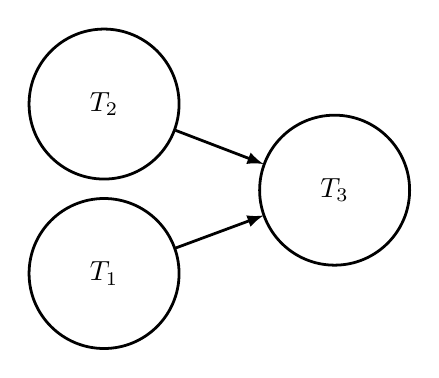
\begin{tikzpicture}[>=latex,line join=bevel,]
  \pgfsetlinewidth{1bp}
%%
\pgfsetcolor{black}
  % Edge: T_2 -> T_3
  \draw [->] (52.743bp,78.531bp) .. controls (59.73bp,75.856bp) and (67.459bp,72.898bp)  .. (84.409bp,66.411bp);
  % Edge: T_1 -> T_3
  \draw [->] (52.743bp,36.164bp) .. controls (59.73bp,38.752bp) and (67.459bp,41.614bp)  .. (84.409bp,47.892bp);
  % Node: T_2
\begin{scope}
  \definecolor{strokecol}{rgb}{0.0,0.0,0.0};
  \pgfsetstrokecolor{strokecol}
  \draw (27bp,88bp) ellipse (27bp and 27bp);
  \draw (27bp,88bp) node {$T_2$};
\end{scope}
  % Node: T_3
\begin{scope}
  \definecolor{strokecol}{rgb}{0.0,0.0,0.0};
  \pgfsetstrokecolor{strokecol}
  \draw (110bp,57bp) ellipse (27bp and 27bp);
  \draw (110bp,57bp) node {$T_3$};
\end{scope}
  % Node: T_1
\begin{scope}
  \definecolor{strokecol}{rgb}{0.0,0.0,0.0};
  \pgfsetstrokecolor{strokecol}
  \draw (27bp,27bp) ellipse (27bp and 27bp);
  \draw (27bp,27bp) node {$T_1$};
\end{scope}
%
\end{tikzpicture}

